%---------------------
% START OF PREAMBLE - do not delete!
%---------------------
\documentclass[12pt]{article}
\usepackage[pdftex]{graphicx}
\usepackage{amsmath}
\usepackage{verbatim}
\DeclareGraphicsRule{*}{mps}{*}{}

%==============================================================================
% Page layout
%==============================================================================

%------------------------------------------------------------------------------
%  Define the page dimensions.
%------------------------------------------------------------------------------
\setlength{\hoffset}{0.0in}
\setlength{\oddsidemargin}{0.0in}
\setlength{\evensidemargin}{0.0in}
\setlength{\textwidth}{6.75in}

\setlength{\voffset}{0in}
\setlength{\topmargin}{-.6in}
\setlength{\headheight}{12pt}
\setlength{\headsep}{12pt}
\setlength{\textheight}{9.5in}
\renewcommand{\baselinestretch}{1.0}
\renewcommand{\labelitemi}{-}

% writing the section number and the subsection number together
% and also the subsubsection in the form of 1.a
\renewcommand\thesubsection{\arabic{section}.\alph{subsection}}
\renewcommand\thesection{Problem \arabic{section}}
%------------------------------------------------------------------------------

%---------------------
% END OF PREAMBLE - do not delete!
%---------------------
\begin{document}

%---------------------
% make the title
%---------------------
\begin{titlepage}
\centering
{\LARGE\bfseries Homework 2}

\vspace{1cm}

{\Large Aerosol Physics, Chemistry, Clouds and Climate}

\vspace{2cm}

{\large Masoud Akbarzadeh}

\vspace{2cm}

{ \today }

\vfill

{\itshape Colorado State University}
\end{titlepage}


%---------------------

%---------------------
% begin main text
%---------------------
\section{Condensation}\label{sec:problem-1}
\subsection{}\label{subsec:problem-1-a}





\subsection{}\label{subsec:problem-1-b}


Since the z-score is greater than the critical value, the null hypothesis is rejected.

\subsection{}\label{subsec:problem-1-c}


%new page
\newpage
\section{Coagulation}\label{sec:problem-2}
% part A of problem 2 % subsection written in form of 2.a
\subsection{Hypothesis testing}\label{subsec:problem-2-a}



\newpage
\subsection{Sensitivity Analysis}\label{subsec:problem-2-c}

Assuming $\gamma$ values are from $0$ to $1$.
For each of gamma, 10000 monte carlo simulations were run.
Then the fraction of time each approach gives the correct answer was calculated.
The results are shown in the figure ~\ref{fig:problem-2-c}.\\
The results show that for all values of $\gamma$, the Bayesian approach is better than the hypothesis testing approach for this problem.
This is because the Bayesian approach is using the prior information about the wind direction.
Also, the Bayesian approach is least effective when $\gamma = 0.5$ while the frequentist approach is least effective when $\gamma = 0$.
The model in the frequentist approach does not have any knowledge about the wind that is coming from the east, and its probability of happening so the model is only effective in $\gamma$ values close to 1 where the most probable wind is from the west.

\newpage

\begin{figure}\label{fig:problem-2-a-1}
\begin{center}
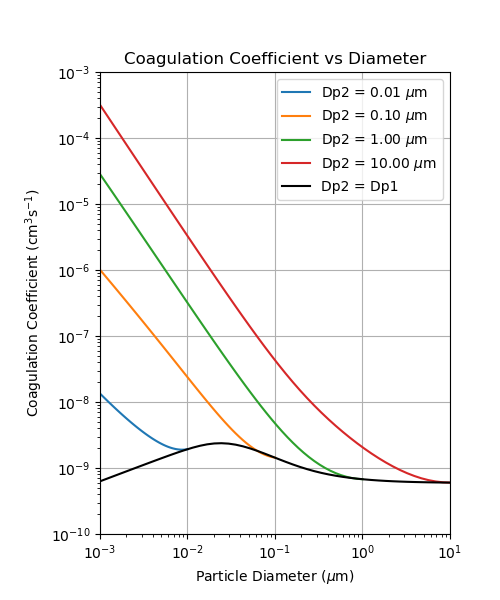
\includegraphics[width=3in]{hw2_pr2_1_coagulation_coefficient_vs_diameter}
\caption{Fuchs Coagulation the code}
\end{center}
\end{figure}

\begin{figure}\label{fig:problem-2-a-2}
\begin{center}
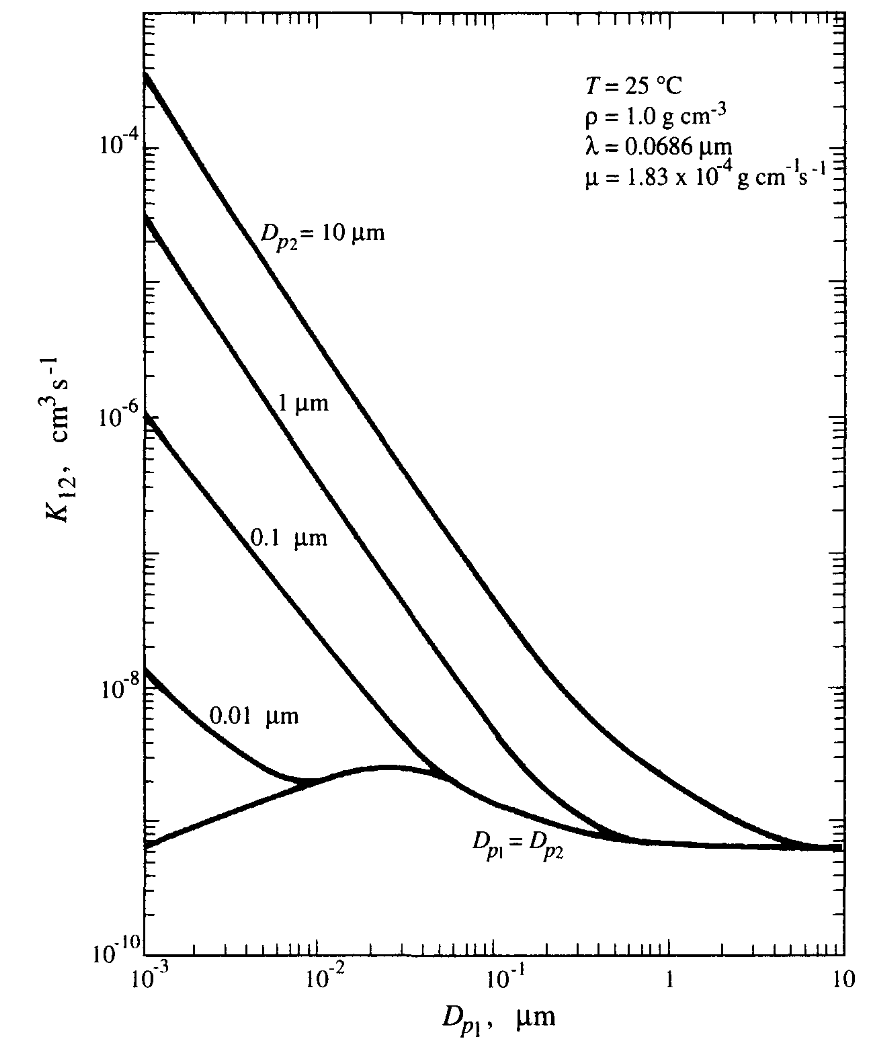
\includegraphics[width=3in]{Table_13_5_Fuchs_Coagulation_plot.png}
\caption{Table\_13\_5 Fuchs Coagulation plot}
\end{center}
\end{figure}



\end{document}


